%%%%%%%%%%%%%%%%%%%%%%%%%%%%%%%%%%%%%%%%%%%%%%%%%%%%%%%%
%   |------------------------------------------|       %
%   | Web App embebida en dispositivos móviles |       %
%   |  para la gestión de registros sobre la   |       %
%   |   contaminación de afluentes y ríos.     |       %
%   |                                          |       %
%   |          Proyecto de graduación          |       %
%   |__________________________________________|       %
%                                                      %
%   Autores                                            %
%   -------                                            %
%                                                      %
% * Bruno, Ricardo Hugo (CX 1409686)                   %
%     rburnount@gmail.com                              %
% * Gómez Veliz, Kevin Shionen (CX 1411828)            %
%     ing.gomezvelizkevin@gmail.com                    %
%                                                      %
%   Tutor                                              %
%   -------                                            %
%                                                      %
% * Ing. Cohen, Daniel Eduardo                         %
%        dcohen.tuc@gmail.com                          %
%                                                      %
%   Cotutor                                            %
%   -------                                            %
%                                                      %
% * Ing. Nieto, Luis Eduardo                           %
%        lnieto@herrera.unt.edu.ar                     %
%                                                      %
%                                                      %
%%%%%%%%%%%%%%%%%%%%%%%%%%%%%%%%%%%%%%%%%%%%%%%%%%%%%%%%

\chapter{Disciplina de Pruebas}
\label{chap:pruebas}

\section{Test de Unidades}
	\subsection{Introducción}

		El Test de Unidades consiste en realizar pruebas de las unidades individuales de código. En esta fase se realizan las pruebas de caja blanca. 

	\subsection{Pruebas de Caja Blanca}
		Es un tipo de método de prueba que permite detectar errores internos del código de cada módulo. 

		Con estas pruebas se pueden garantizar que se ejercitan por lo menos una vez todos los caminos independientes de cada módulo, que las decisiones lógicas se evalúan en sus dos variantes (verdadera y falsa), que se ejecutan todos los bucles en sus límites operacionales y que se ejercitan las estructuras internas de datos para asegurar su validez.
		\newline

		\textbf{Pruebas realizadas:}
		Para el mantenimiento del código, se implementaron test unitarios por módulos, para asegurarse que el código este siempre funcionando correctamente. Algunos de los módulos con test unitarios son: formulario para alta usuario, formulario para nuevos registros, entre otros.
		Todos estos test son usados para controlar la integridad de los datos ingresados.

\section{Test de Módulos}

	\subsection{Introducción}
		El Test de Módulos consiste en realizar pruebas de los módulos funcionales del sistema. En esta fase se realizan las pruebas de caja negra y las pruebas de estrés. 

	\subsection{Pruebas de Caja Negra}

		En este método de prueba se ve a cada módulo como una caja negra y se generan conjuntos de condiciones de entrada que ejerciten completamente todos los requisitos funcionales del programa, observando las salidas.

		Con estas pruebas se pueden detectar funciones incorrectas o ausentes, errores de interfaz, errores de rendimiento, etc.
		\newline

		\textbf{Pruebas realizadas:}
		Al finalizar los módulos, se realizaron los test de caja negra correspondientes, validando así que la entradas de datos genere la salida esperada.
		Por ejemplo, al crear un registro, si no se capturo la foto de la muestra, el usuario recibe el correspondiente mensaje de error. Esta acción se realiza para los requisitos obligatorios de un registro, hasta comprobar su validez, para luego ser guardado en la base de datos.
			
	\subsection{Pruebas de Estrés}

		Esta prueba se centra en realizar el análisis de valores límites, y en condiciones límites, ya que se ha demostrado que los errores tienden a darse más en los límites del campo de entrada y sometidos a condiciones límites.

		\newpage
		\textbf{Pruebas realizadas:}
		Para las pruebas de estrés se sometió a la base de datos no relacional (couchDB) a la creación de 100 registros prototipo, donde obtuvieron los siguientes resultados no satisfactorios:
		\begin{itemize}
			\item Demora en la sincronización entre las BD.
			\item Falla en la sincronización.
			\item La BD crecía exponencialmente su tamaño debido al versionado nativo de los documentos al actualizarlos.
		\end{itemize}
		Por estos motivos, se rediseño el sistema para trabajar con una BD Relacional (MySql) realizando los siguientes cambios:
		\begin{itemize}
			\item Se modifico el protocolo de comunicación entre el sistema y el servidor
			\item Se creo un protocolo de sincronización automática que se ajusta a los requisitos del sistema
			\item Se implemento web socket para ver los cambios de la sincronización en tiempo real.
		\end{itemize}
		
		\textbf{Pruebas realizadas con el rediseño:}

		Se realizaron las mismas pruebas, pero esta vez, con resultados satisfactorios para todos los puntos enunciados anteriormente.


\section{Test de Integración}

	\subsection{Introducción}

		El Test de Integración consiste en realizar pruebas de la estructura modular del programa y su interacción a través de la prueba de integración.

	\subsection{Pruebas de Integración}

		En este tipo de prueba los errores surgen al integrar los módulos. En esta fase se pueden detectar errores como por ejemplo que las subfunción, es cuando se combinan pueden no producir la función principal, un módulo puede tener un efecto adverso e inadvertido sobre otro, etc.

		El objetivo es tomar los módulos probados y construir una estructura de programa que esté de acuerdo con lo que dicta la especificación C.
			
		Existen dos tipos de integración:
			\begin{itemize}
				\item \textbf{Integración descendente:} En este tipo se integran los módulos moviéndose hacia abajo por la jerarquía de control, comenzando con el módulo de control inicial.
				\item \textbf{Integración ascendente:} En este tipo se integran los módulos atómicos primero y luego se continúa con el nivel inmediato superior.
			\end{itemize}

	En el desarrollo de este sistema se utilizó la integración descendente. Probando a mano, todos los casos escenarios posibles, como por ejemplo:
	\begin{itemize}
		\item Creación de registros.
		\item Iniciar sesión
		\item Comprobar el estado del mapa general, con los registros validados.
		\item Acceder al perfil
	\end{itemize}
	Todos estos casos fueron probados de manera online y offline.
	En funciones como ver el mapa general, que requieren conexión a internet y nos encontramos offline, se muestra un mensaje de alerta y no se permite el acceso a dicha función. Por otro lado, funciones que no requieren conexión a internet, de manera offline, pueden ser accedidas sin problemas

\section{Test de Aceptación}

	\subsection{Introducción}

		El Test de Aceptación consiste en realizar la prueba del software para validar si funciona de acuerdo con las expectativas razonables del cliente. En esta fase se llevan a cabo las pruebas Alfa y Beta.

	\subsection{Prueba Alfa}

		Esta prueba es conducida por el cliente en el lugar de desarrollo. Se usa el software de forma natural (previa capacitación), con el encargado de desarrollo mirando “por encima del hombro” del usuario y registrando errores y problemas de uso. Se lleva acabo en un entorno controlado.

		\textbf{Conclusiones de estas pruebas:}
		Tras esta prueba, nos dimos cuenta de algunos errores y posibles mejoras, no solo de funcionamiento, sino también de la interfaz de usuario, ya que no era muy amigable. 
		Para esta prueba se realizó una salida de campo real con el cliente (docente Daniel Dos Santos), en la cual pudimos apreciar que nuestro sistema cumplió correctamente con los requisitos planteados.
		Esta prueba se realizó con un smartphone de gama baja, y aun así, obtuvimos fotos legibles, coordenadas del GPS correctas, fluidez en la interfaz de usuario y un buen \textit{performance} del dispositivo móvil en lo se refiere a procesamiento, creación y guardado de los registros.
		\newpage 

		\textbf{Fotos de la salida de campo:}

		\begin{figure}[H]
			\centering
				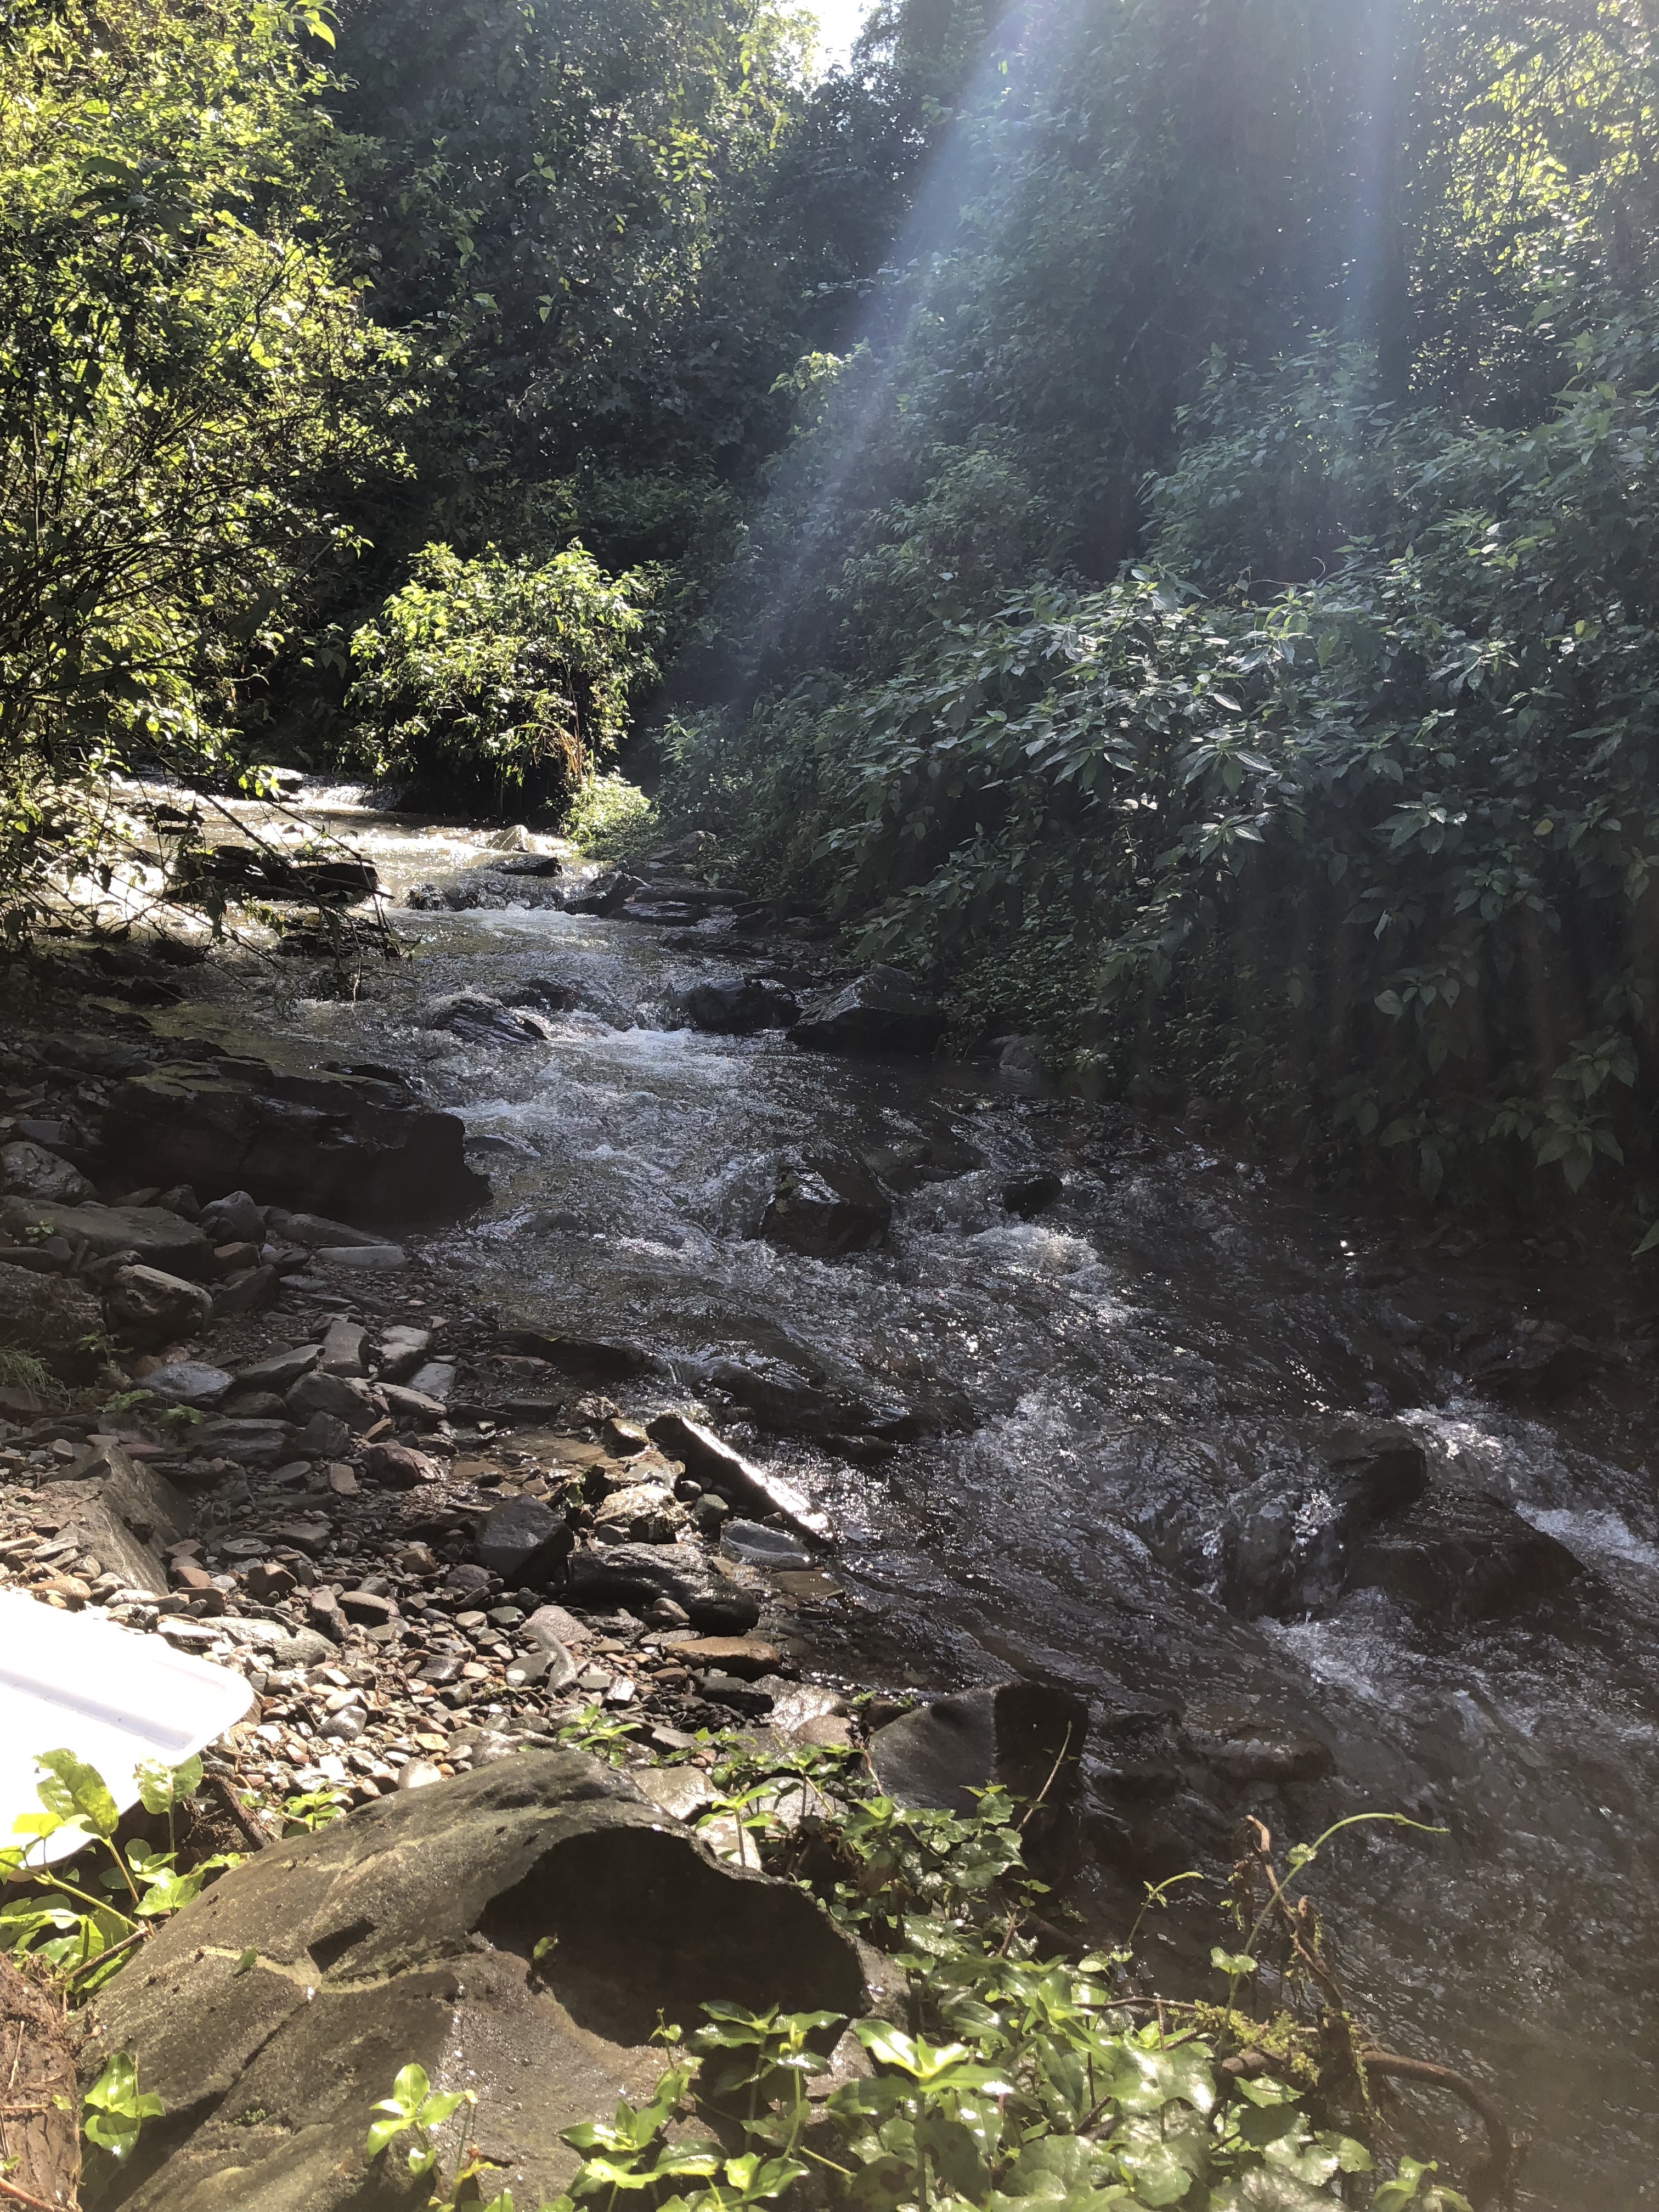
\includegraphics[width=0.9\textwidth]{imagenes/testAlpha/1.JPG}
					\caption{Foto paisaje de la muestra que sirve para futuro reconocimiento}
		\end{figure}
		\begin{figure}[H]
			\centering
				\includegraphics[width=0.9\textwidth]{imagenes/testAlpha/2.JPG}
					\caption{Red de pie utilizada para la obtención de la muestra}
		\end{figure}
		\begin{figure}[H]
			\centering
				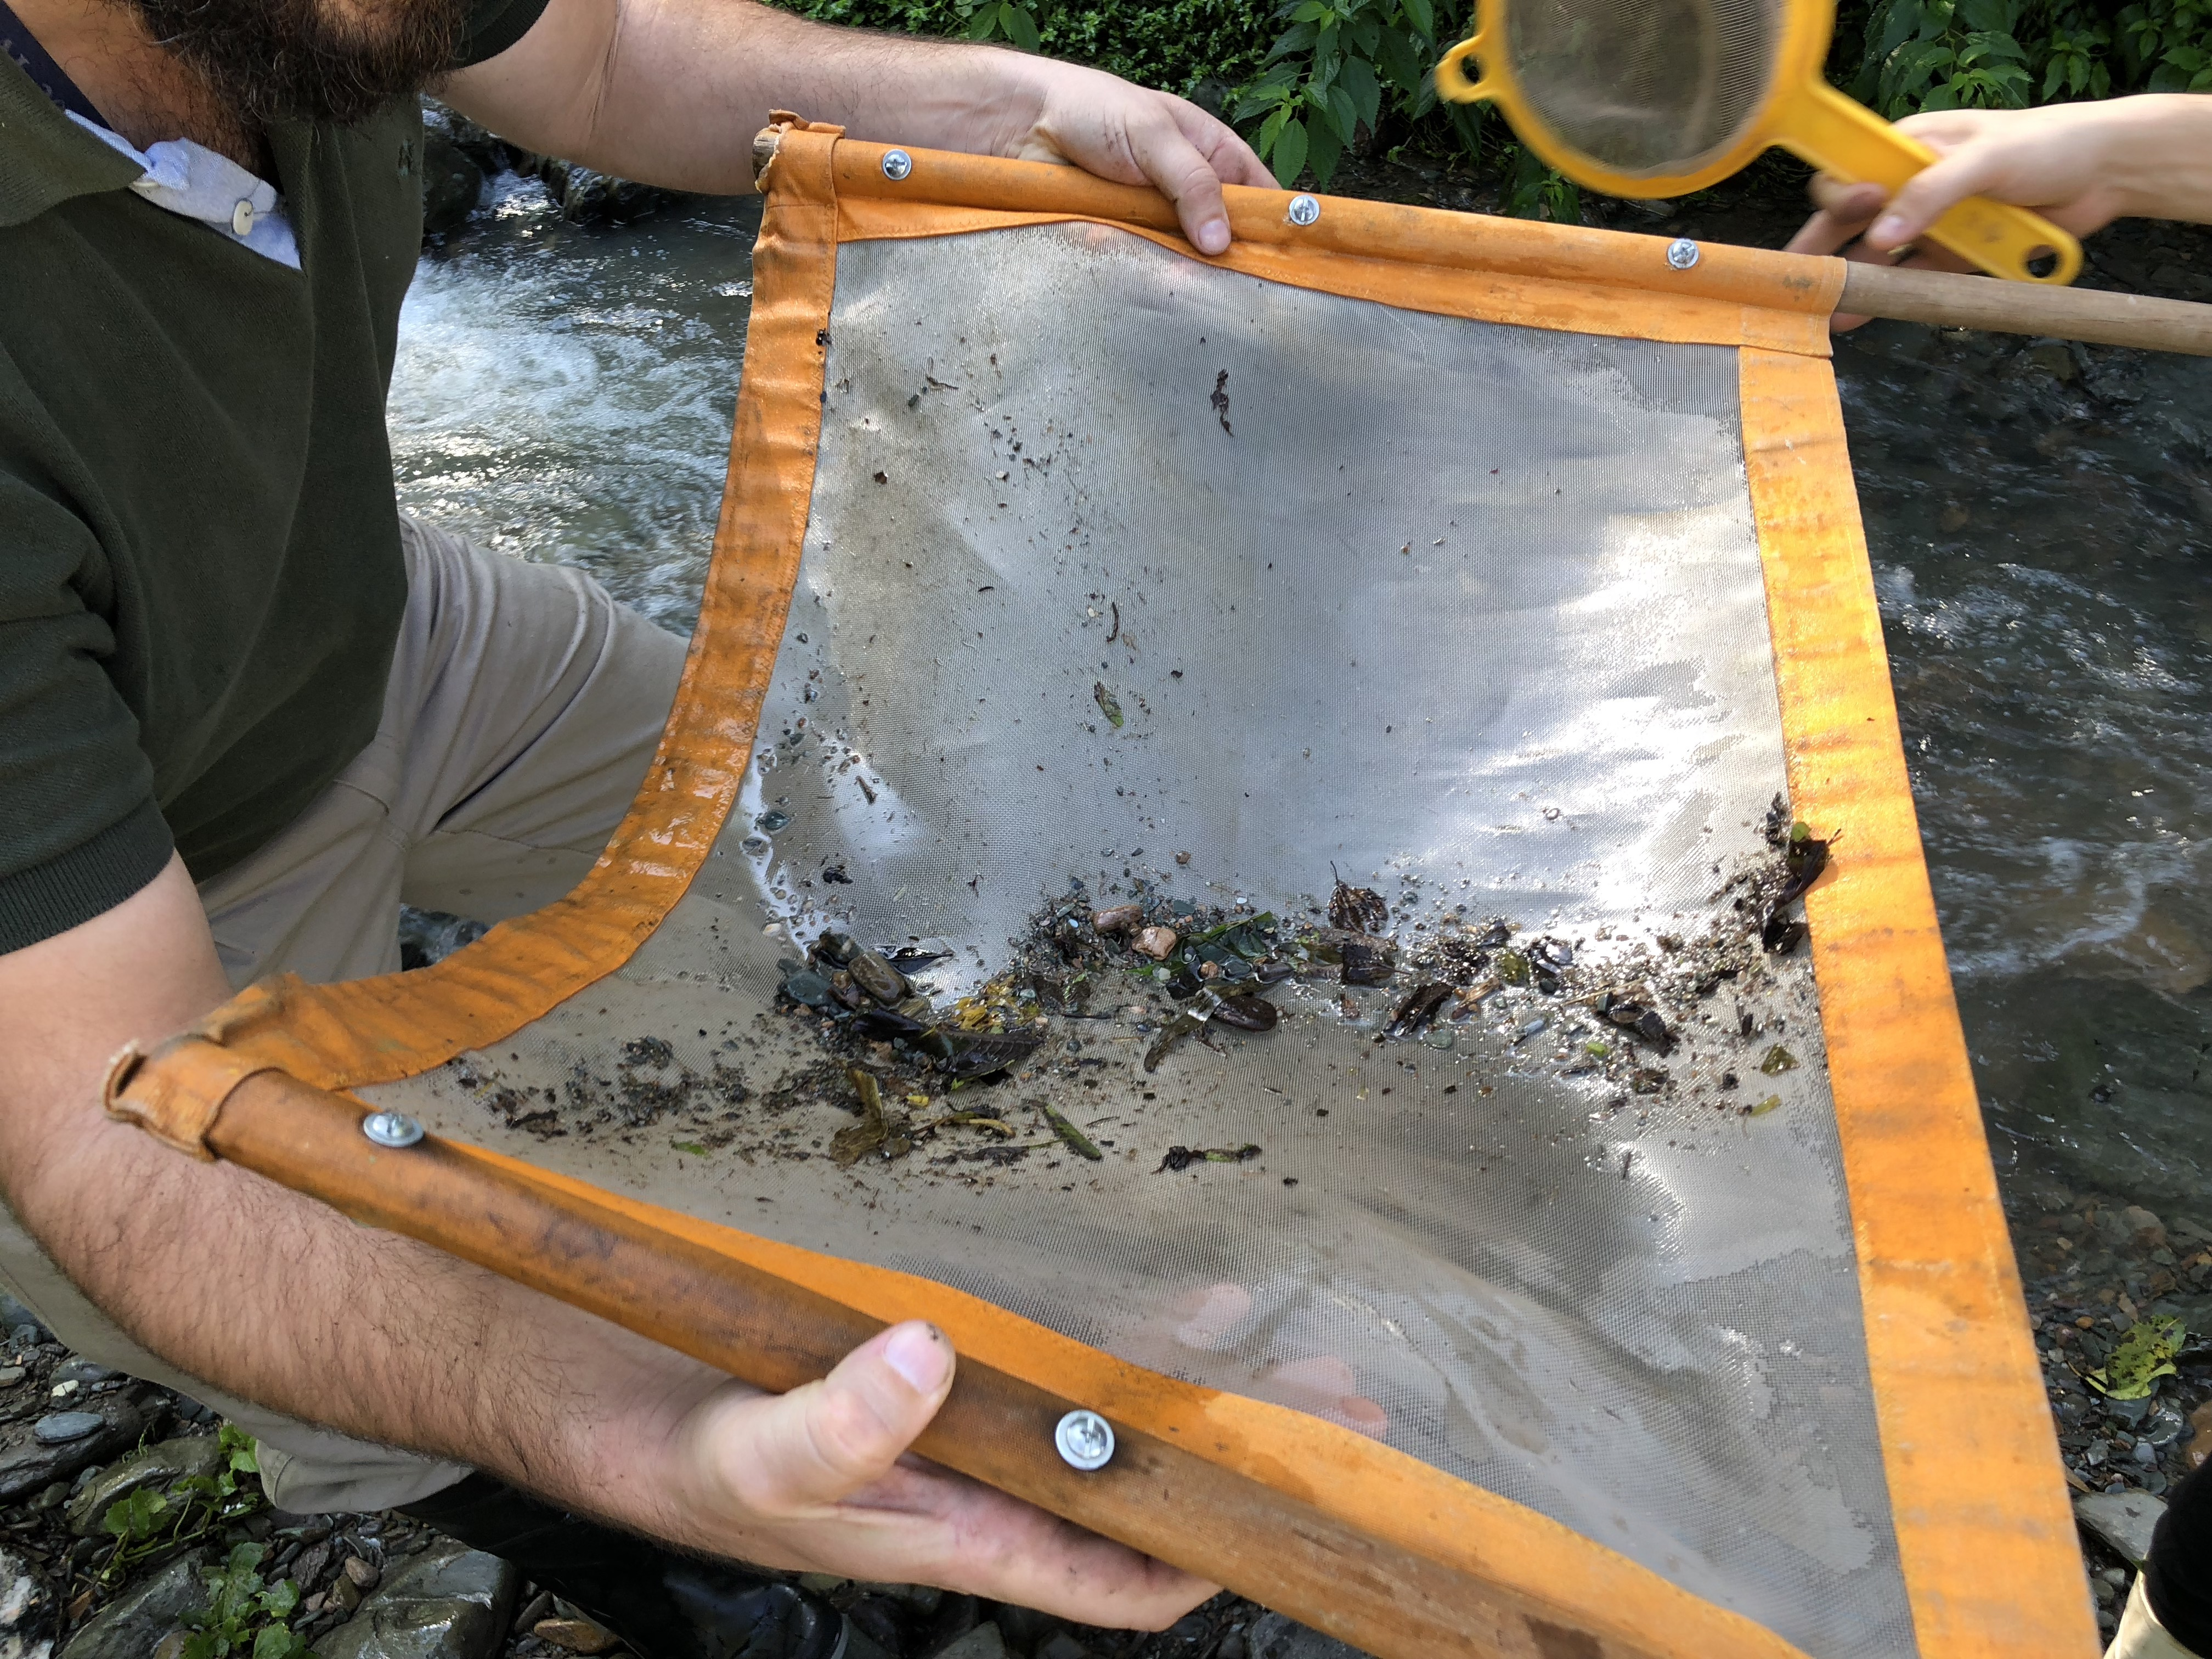
\includegraphics[width=0.9\textwidth]{imagenes/testAlpha/3.JPG}
					\caption{Proceso de validación de la muestra}
		\end{figure}
		\begin{figure}[H]
			\centering
				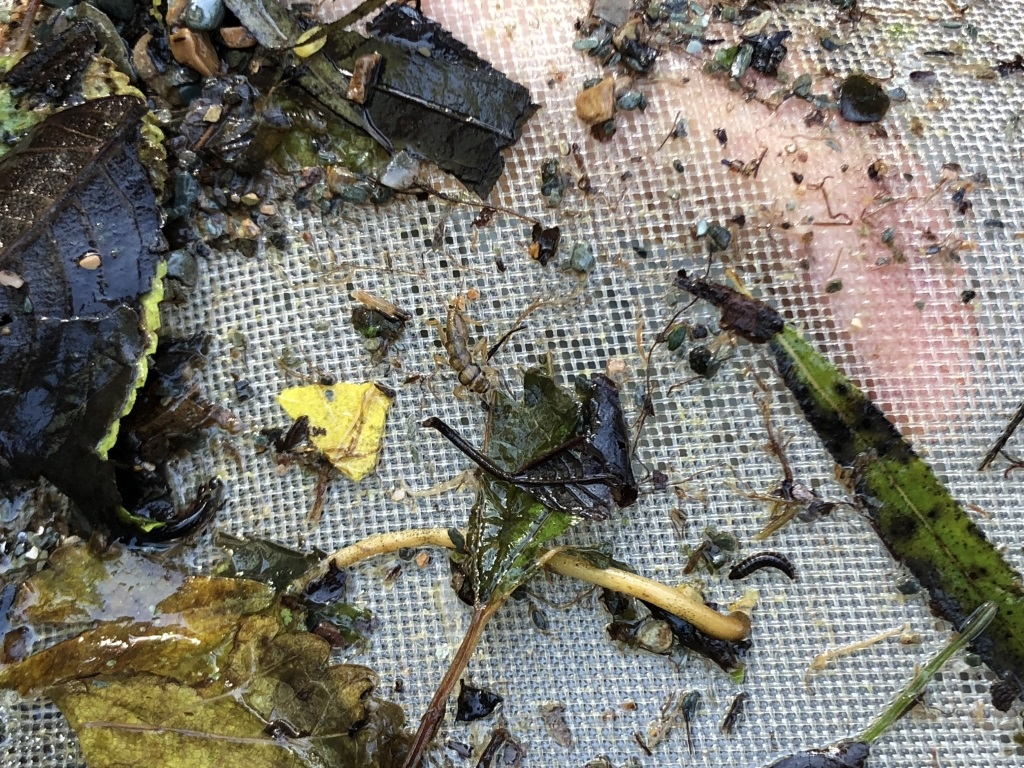
\includegraphics[width=0.9\textwidth]{imagenes/testAlpha/4.JPG}
					\caption{Proceso de identificación y extracción de los insectos objetivos}
		\end{figure}
		\begin{figure}[H]
			\centering
				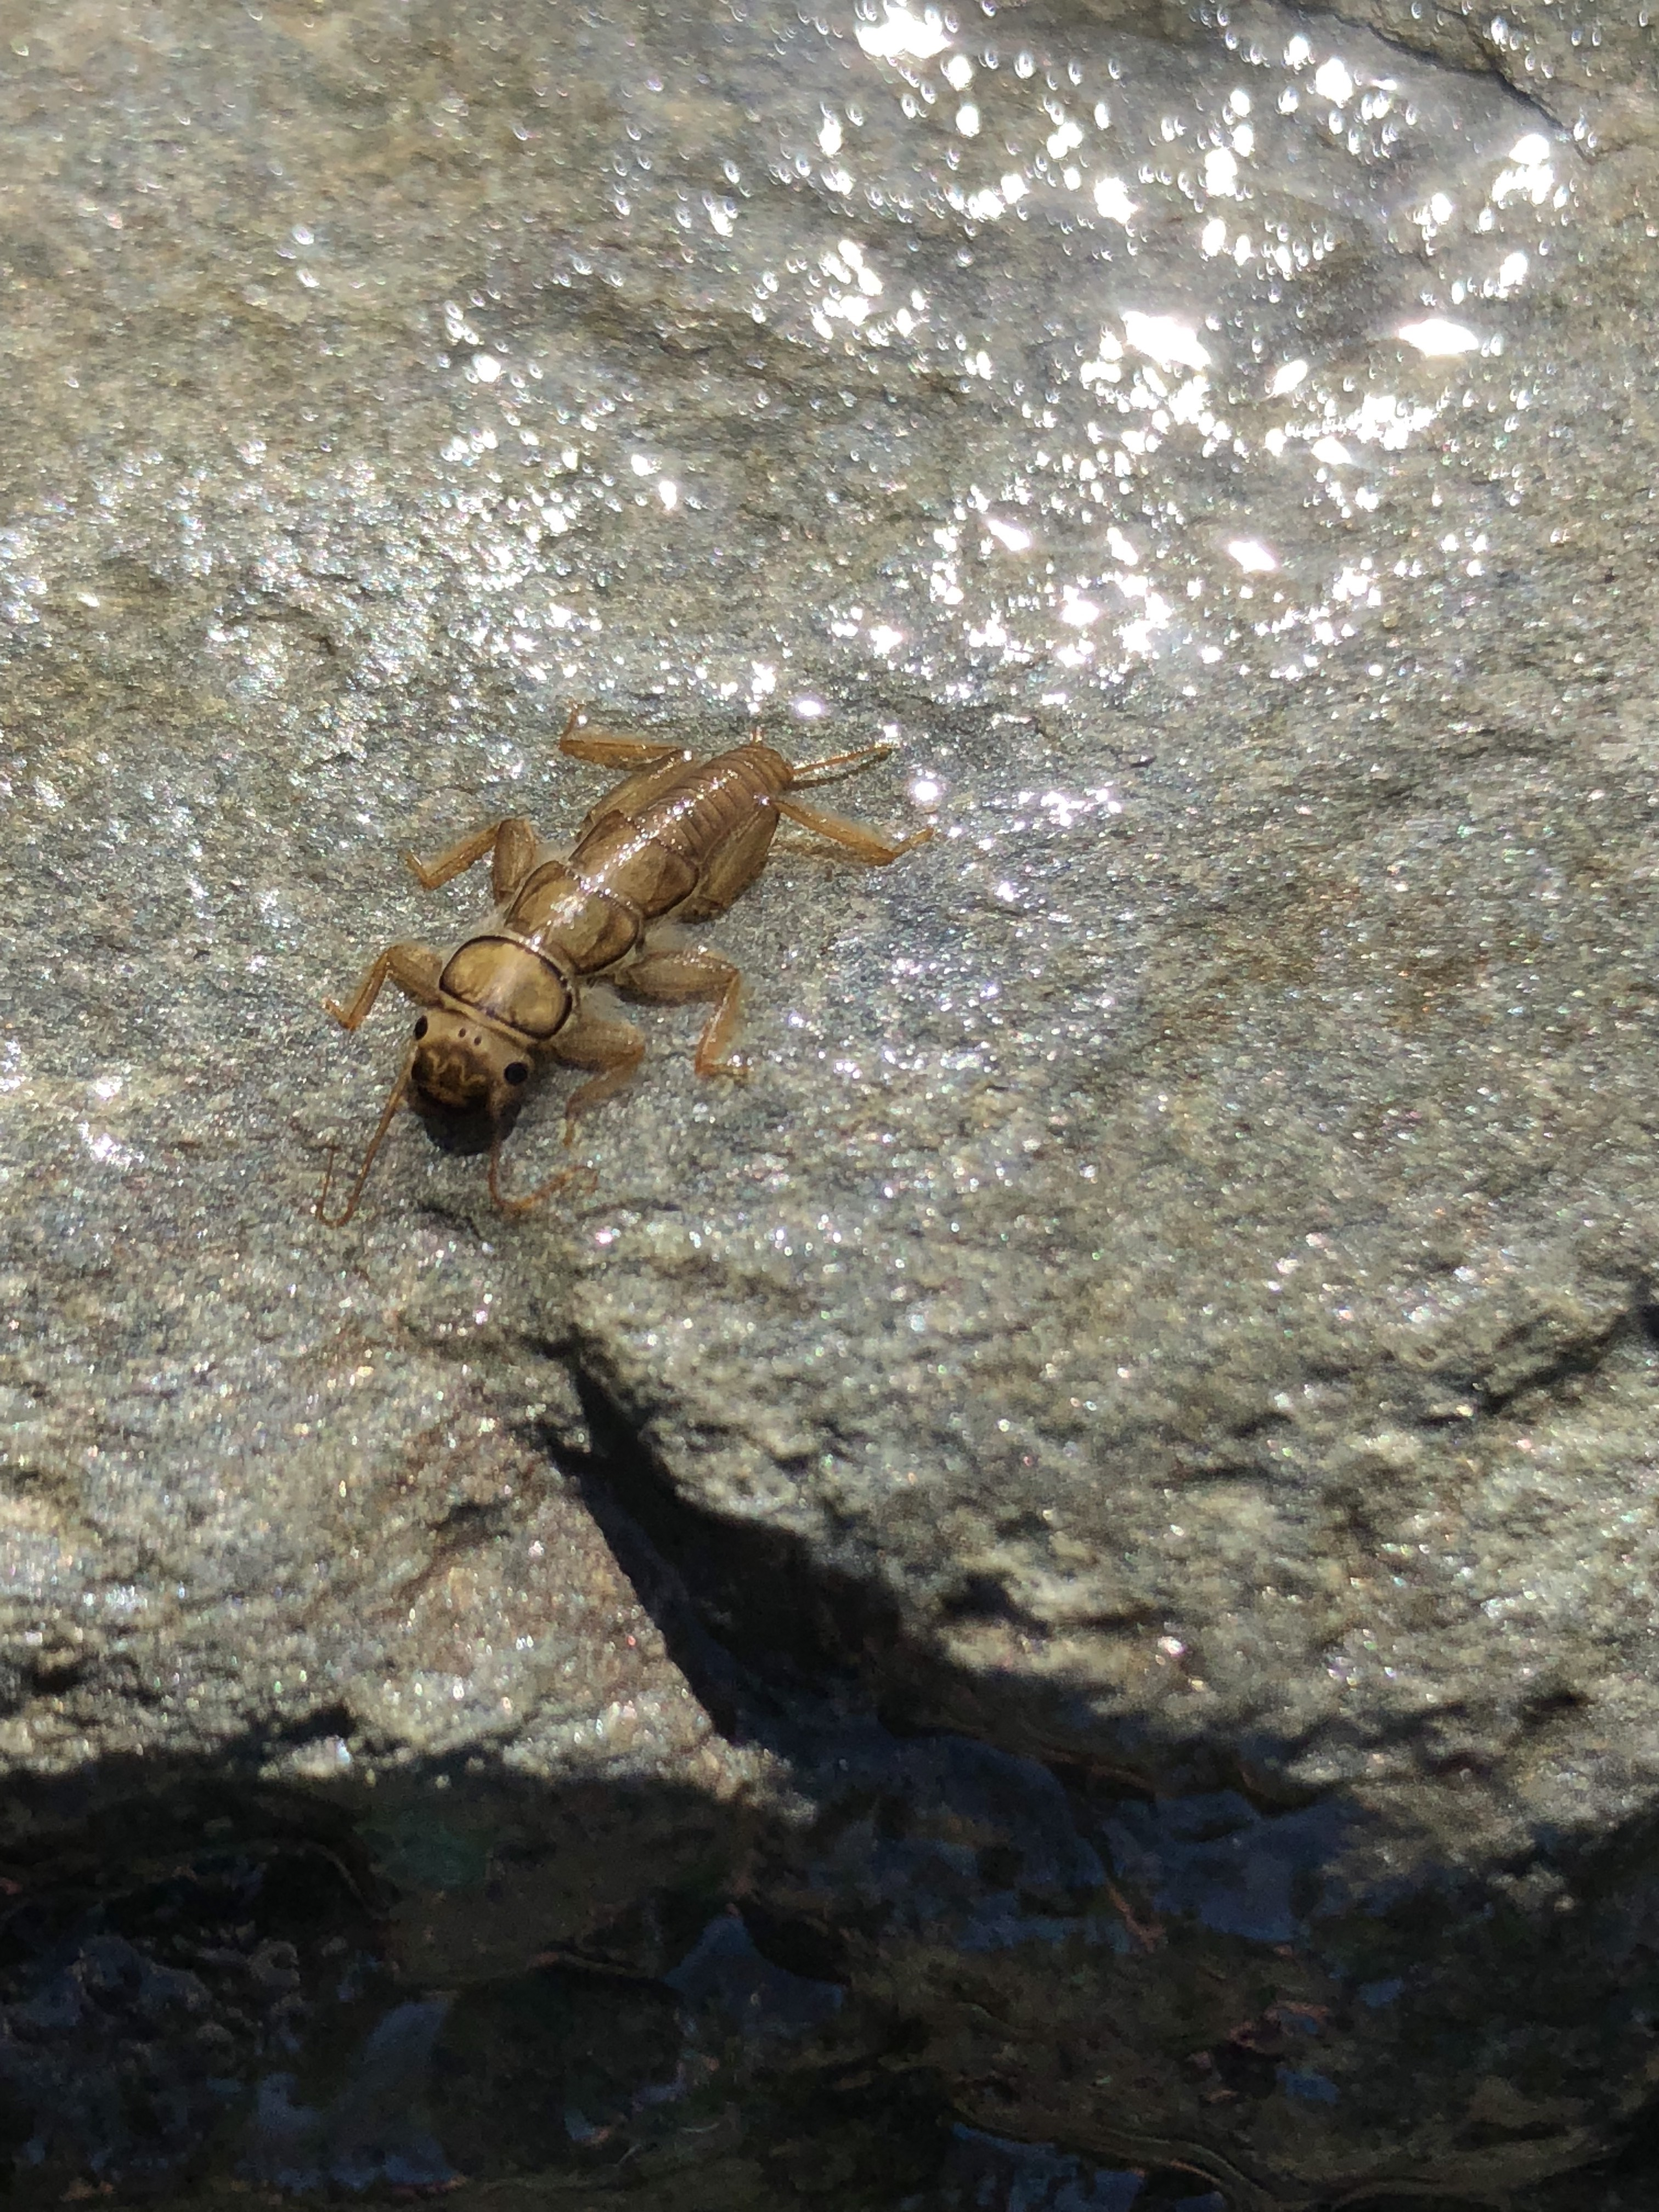
\includegraphics[width=0.9\textwidth]{imagenes/testAlpha/5.JPG}
					\caption{Foto real del insecto \textit{Plecoptero}}
		\end{figure}
		\begin{figure}[H]
			\centering
				
\includegraphics[width=0.9\textwidth]{imagenes/testAlpha/6.JPG}
					\caption{Foto real del insecto \textit{Patudo}}
		\end{figure}
		
	\subsection{Prueba Beta}

		Esta prueba se lleva a cabo en uno o más lugares de clientes, por los usuarios finales de software. El encargado de desarrollo no está presente. El cliente registra todos los problemas (reales o imaginarios) que  encuentra durante la prueba o informa a intervalos regulares al equipo de desarrollo. Se lleva a cabo en un entorno no controlado.

		Los procedimientos de prueba se diseñaron para asegurar que se satisfacen todos los requisitos funcionales y que se alcanzan todos los requisitos de rendimiento.
		\newline

		\textbf{Pruebas realizadas:}
		
		No se realizaron las pruebas betas, sin embargo se programo una para finales de octubre del 2018, con la participación de los alumnos de escuelas rurales (usuario final del sistema).
